\documentclass[11pt,letterpaper]{article}

\usepackage{fancyhdr}
\usepackage{lastpage}
\usepackage[T1]{fontenc}
\usepackage[latin1]{inputenc}
\usepackage[cyr]{aeguill}
\usepackage[colorlinks=true]{hyperref}
\usepackage{textpos}
\usepackage{graphicx}
\usepackage[english]{babel}
\usepackage{color}
\usepackage{array}
\usepackage{enumitem}
\usepackage{amsmath}
\usepackage{amssymb}
\usepackage{amsthm}
\usepackage{multicol}   % For side-by-side formatting

\usepackage{framed}
%\usepackage{enumerate}
\definecolor{shadecolor}{gray}{0.9}

\usepackage{xcolor}

\definecolor{problemcolor}{rgb}{0.2, 0.1, 0.8} % Define color for Problem
\definecolor{solproblemcolor}{rgb}{0.8, 0.2, 0.2} % Define color for Solution to Problem

\theoremstyle{definition}
\newtheorem{prob}{\textcolor{problemcolor}{Problem}}  % Color for Problem
\newtheorem{solprob}{\textcolor{solproblemcolor}{Solution to Problem}}  % Col

\usepackage[letterpaper, left=25mm, right=25mm, top=20mm, bottom=30mm]{geometry}
\usepackage{amsmath}
\usepackage{amssymb}
\usepackage{amsfonts}
\usepackage{dsfont}
\usepackage{amsthm}
\usepackage{float}


%\usepackage{enumerate}
\usepackage{fancyhdr}
\pagestyle{fancy}


\renewcommand{\headrulewidth}{0pt}
\renewcommand{\footrulewidth}{4pt}
\allowdisplaybreaks


\newcommand{\session}{Fall 2025}




\def\0{{\mathbf 0}}
\def\1{{\mathbf 1}}

\def\a{{\mathbf a}}
\def\b{{\mathbf b}}
\def\c{{\mathbf c}}
\def\d{{\mathbf d}}
\def\e{{\mathbf e}}
\def\f{{\mathbf f}}
\def\g{{\mathbf g}}
\def\h{{\mathbf h}}
\def\i{{\mathbf i}}
\def\j{{\mathbf j}}
\def\k{{\mathbf k}}
\def\l{{\mathbf l}}
\def\m{{\mathbf m}}
\def\n{{\mathbf n}}
\def\o{{\mathbf o}}
\def\p{{\mathbf p}}
\def\q{{\mathbf q}}
\def\r{{\mathbf r}}
\def\s{{\mathbf s}}
\def\t{{\mathbf t}}
\def\u{{\mathbf u}}
\def\v{{\mathbf v}}
\def\w{{\mathbf w}}
\def\x{{\mathbf x}}
\def\y{{\mathbf y}}
\def\z{{\mathbf z}}

\def\A{{\mathbf A}}
\def\B{{\mathbf B}}
\def\C{{\mathbf C}}
\def\D{{\mathbf D}}
\def\E{{\mathbf E}}
\def\F{{\mathbf F}}
\def\G{{\mathbf G}}
\def\F{{\mathbf F}}
\def\H{{\mathbf H}}
\def\I{{\mathbf I}}
\def\J{{\mathbf J}}
\def\K{{\mathbf K}}
\def\L{{\mathbf L}}
\def\M{{\mathbf M}}
\def\N{{\mathbf N}}
\def\O{{\mathbf O}}
\def\P{{\mathbf P}}
\def\Q{{\mathbf Q}}
\def\R{{\mathbf R}}
\def\S{{\mathbf S}}
\def\T{{\mathbf T}}
\def\U{{\mathbf U}}
\def\V{{\mathbf V}}
\def\W{{\mathbf W}}
\def\X{{\mathbf X}}
\def\Y{{\mathbf Y}}
\def\Z{{\mathbf Z}}


\def\rE{{\text{E}}}
\def\rPr{{\text{Pr}}}
\def\Tr{{\text{Tr}}}
\def\vec{{\textrm{vec}}}
\def\ie{{\textit{i.e.}}}
\def\eg{{\textit{e.g.}}}


\def\cA{{\mathcal A}}
\def\cB{{\mathcal B}}
\def\cC{{\mathcal C}}
\def\cD{{\mathcal D}}
\def\cE{{\mathcal E}}
\def\cF{{\mathcal F}}
\def\cG{{\mathcal G}}
\def\cH{{\mathcal H}}
\def\cI{{\mathcal I}}
\def\cK{{\mathcal K}}
\def\cL{{\mathcal L}}
\def\cM{{\mathcal M}}
\def\cN{{\mathcal N}}
\def\cO{{\mathcal O}}
\def\cP{{\mathcal P}}
\def\cQ{{\mathcal Q}}
\def\cR{{\mathcal R}}
\def\cS{{\mathcal S}}
\def\cT{{\mathcal T}}
\def\cU{{\mathcal U}}
\def\cV{{\mathcal V}}
\def\cW{{\mathcal W}}
\def\cX{{\mathcal X}}
\def\cY{{\mathcal Y}}
\def\cZ{{\mathcal Z}}


\def\bphi{{\pmb{\phi}}}
\def\bpsi{{\pmb{\psi}}}
\def\bphi{{\pmb{\phi}}}
\def\bpsi{{\pmb{\psi}}}
\def\balpha{{\boldsymbol \alpha}}
\def\bbeta{{\boldsymbol \beta}}
\def\bvarphi{{\boldsymbol \varphi}}
\def\bPhi{{\boldsymbol \Phi}}


\def\bcdot{{\;\boldsymbol{\cdot}\;}}


%\oddsidemargin 0pt
%\topmargin 0pt
%\textwidth 6.5in
%\textheight 8.1in
\newtheorem{exemple}{Exemple}

\definecolor{bleu_poly}{RGB}{65,170,230}
\definecolor{vert_poly}{RGB}{140,200,60}
\definecolor{orange_poly}{RGB}{250,150,30}
\definecolor{rouge_poly}{RGB}{185,30,50}
\definecolor{gris_poly}{RGB}{166,168,171}

\newcommand{\matlab}{\textsc{Matlab} }
\newcommand{\simulink}{\textsc{Simulink} }

\title{\vspace{-5.5cm} \noindent\makebox[\linewidth]{\color{rouge_poly}{\rule{\textwidth}{1.5pt}}}
	\begin{center}
		\begin{tabular}{m{8cm}m{7cm}}
			\textbf{ \huge Homework 3}  & 
\includegraphics[width=0.4\textwidth]{York_logo}
		\end{tabular}
	\end{center}
	\noindent\makebox[\linewidth]{\color{rouge_poly}{\rule{\textwidth}{1.5pt}}}
	\\ \ \\
	\LARGE EECS 2200 - Electrical Circuits}\vspace{0.01mm}


\author{\session\vspace{3mm} \\ Departement of Electrical Engineering and Computer Science \\\vspace{8mm}
	York University\\
	\textbf{Instructor:} Houshang Karimi}

\date{\textbf{Due Date:} November 10, 2025\\[5mm]
	\textbf{Last Update:} \today}





\pagestyle{fancy}

\usepackage{lastpage}
%\rfoot{Page \thepage~of \pageref{LastPage}}

\lfoot{\session}
\cfoot{~~~~~~~EECS 2200 - Electrical Circuits ~~~~~~~ Page \thepage~of \pageref{LastPage}}




\chead{}
\lhead{\emph{Homework 3}}
\rhead{\includegraphics[width=3.5cm]{York_Logo}}
%\rhead{\vspace{-1cm}\includegraphics[width=2cm]{polytechnique_genie_droite_fr_cmyk}}
\renewcommand{\headrulewidth}{0.4pt}
\renewcommand{\footrulewidth}{0.4pt} 
\setlength{\headheight}{45pt}

\graphicspath{{Fig/}}

\newcounter{numq}
\setcounter{numq}{1}    % Value is 0

%\setenumerate[1]{label=(\alph*), leftmargin=3em}

\begin{document}
	\maketitle
	\vspace{-5mm}

%\noindent\makebox[\linewidth]{\color{rouge_poly}{\rule{\textwidth}{1.3pt}}}
%%%%	******************%
%\noindent\textbf{Note:} Writing your homework in \textbf{LaTeX} will be rewarded with bonus points! 

%\begin{enumerate}[label=(\roman*)]
%	\item Writing your homework in \textbf{LaTeX} will be rewarded with bonus points! 
%	\item Submit your MATLAB simulation files (.m files) along with your homework solutions. 
%\end{enumerate} 
\noindent\makebox[\linewidth]{\color{rouge_poly}{\rule{\textwidth}{1.3pt}}}	
%%%%	******************%
	
	\vspace{5mm}
	
	\centering
	\fbox{\begin{minipage}{30em}
			\vspace{4mm}
			First Name: Thomas\\\vspace{2mm}
			
			Last Name: Newman\\\vspace{2mm}
			
			Student Number: 221224662
			\vspace{3mm}
	\end{minipage}}
	
	\vspace{-0.1mm}
	
	%\centering
\begin{table}[!h]
	\centering
	\renewcommand{\arraystretch}{2.5}
	\resizebox{0.95\textwidth}{!}{ % Adjust 0.95 to a smaller value to reduce width
		\begin{tabular}{|l|l|l|l|l|l|l|l|l|l|l|l|l|l|l|l|l|l|l|}
			\cline{1-18}
			Problem		& $P_1$ & $P_2$ & $P_3$ & $P_4$  & $P_5$  & $P_6$ &  $P_7$  & $P_8$ &  $P_9$  & $P_{10}$  & $P_{11}$  &  $P_{12}$  &  $P_{13}$  &  $P_{14}$  & $P_{15}$  & $P_{16}$  &   Total  \\ \cline{1-18}
			Mark	    	&  $\dfrac{}{~5~}$ &  $\dfrac{}{~5~}$ &  $\dfrac{}{~5~}$ &  $\dfrac{}{~5~}$ & $\dfrac{}{~5~}$ & $\dfrac{}{~5~}$  & $\dfrac{}{~5~}$   & $\dfrac{}{~5~}$   & $\dfrac{}{~5~}$   & $\dfrac{}{~5~}$   & $\dfrac{}{~5~}$   & $\dfrac{}{~5~}$   &$\dfrac{}{~5~}$   &$\dfrac{}{~5~}$   &$\dfrac{}{~5~}$   & $\dfrac{}{~5~}$   &  $\dfrac{}{~80~}$ \\ \cline{1-18}
		\end{tabular}
	}
	\renewcommand{\arraystretch}{1}
\end{table}

	\noindent\makebox[\linewidth]{\color{rouge_poly}{\rule{\textwidth}{1.5pt}}}
	
\begin{enumerate}
	\item[{\textbf{CLO1:}}] \textbf{Analyze resistive circuits using basic laws (node and loop analysis, Thevenin, Norton's, superposition).}
	\item[{\textbf{CLO2:}}] \textbf{Determine the transient response of RC, RL, and RLC circuits.}
	\item[{\textbf{CLO3:}}] \textbf{Analyze AC circuits in steady state using the phasor method.}
	\item[{\textbf{CLO4:}}] \textbf{Use basic tools such as MATLAB and SPICE for circuit analysis.}
	\item[{\textbf{CLO5:}}] \textbf{Measure basic electrical signals using electronic measurement equipment in a lab setting.}
\end{enumerate}

	\noindent\makebox[\linewidth]{\color{rouge_poly}{\rule{\textwidth}{1.5pt}}}
	\newpage
	
%%% Midterm (Neda) - Fall 2023
\begin{prob}\label{pb:op1}\text{} 
	Consider the op-amp circuit shown in Fig.~\ref{fig:op1}, and assume ideal op-amps.
	\begin{enumerate}[label=(\alph*)]
		\item Calculate the output voltage $V_o$.
		\item Discuss any potential issue with this result for real (non-ideal) op-amps.
	\end{enumerate}

	\vspace{-4mm}
	\begin{figure}[H]
		\centering
		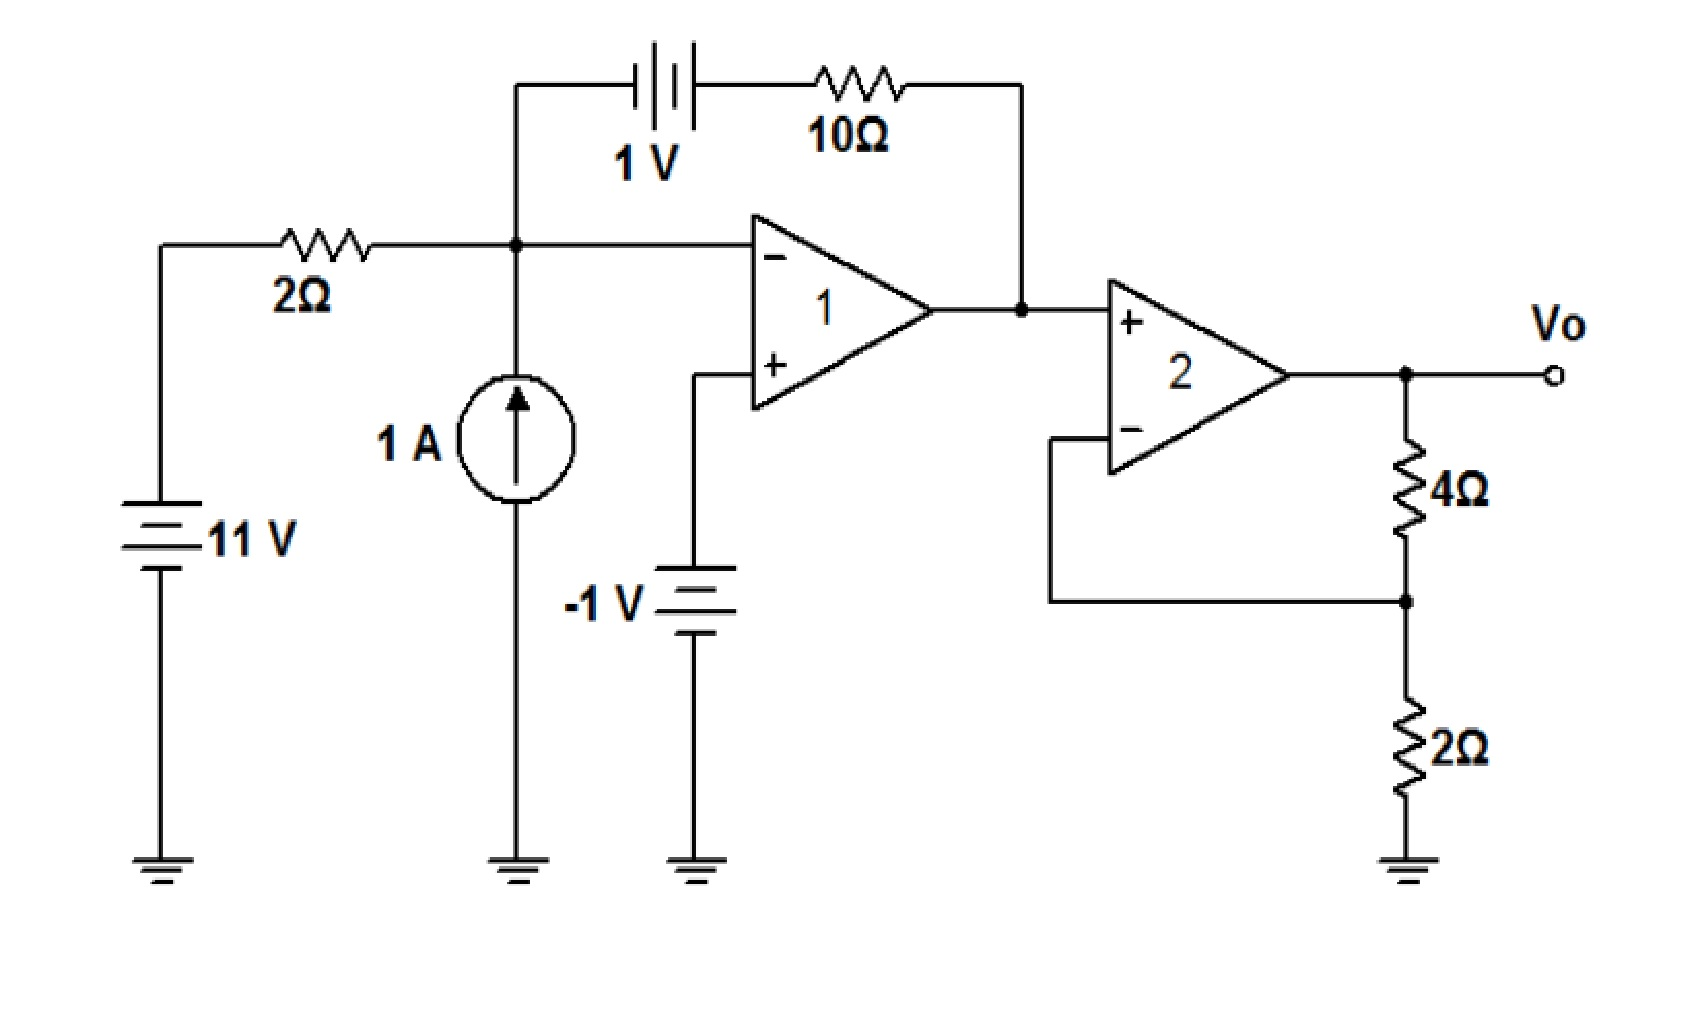
\includegraphics[width=0.7\textwidth]{Fig_OP1.jpg}
		\vspace{-4mm}
		\caption{Op-amp circuit for Problem~\ref{pb:op1}.}
		\label{fig:op1}
	\end{figure}
\end{prob}

\noindent\makebox[\linewidth]{\color{rouge_poly}{\rule{\textwidth}{1.3pt}}}

\begin{solprob}
    (a) Let's begin by focusing on the first op-amp on the right.  We know that $V_n = V_p$ in op-amp circuits. I am also defining the output of the first amp to be $V_x$. First, lets do a KCL on the right op-amp.
    \[V_n=V_p = V_x\]
    \[\text{KCL 1: }\frac{V_o-V_x}{4}+\frac{-V_x}{2}=0\]
    Now, we just need to solve for the output of the first op-amp to solve for $V_o$.  Let's go back to the first op-amp and also do a KCL.
    \[V_p=V_n \implies V_n=-1\]
    \[\text{KCL 2: } i_a +i_b+1=i_n=0\]
    \[\frac{11-V_n}{2}+\frac{V_x-1-V_n}{10}+1=0\]
    \[\frac{12}{2} + \frac{V_x}{10}+1=0\]
    \[70+V_x=0\]
    \[V_x=70\text{ V}\]
    Now, plug our value back into our first equation.
    \[\frac{V_o-(-70)}{4}+\frac{-(-70)}{2}=0\]
    \[\frac{V_o+70}{4} + 35 =0\]
    \[V_o+70+140=0\]
    \[V_o=-210\text{ V}\]
    (b) $V_o$ is too high for a non-ideal amplifier, and is not feasible.  This would likely mean that the amplifier is over-saturated and the output would instead be equal to the magnitude of $V_\text{CC}$.
\end{solprob}
\vspace{-4mm}
\noindent\makebox[\linewidth]{\color{rouge_poly}{\rule{\textwidth}{1.3pt}}}	

%%%% Final Exam (Neda) - Fall 2023
\begin{prob}\label{pb:op2}\text{}
	Calculate the current $I_o$ in the circuit shown in Fig.~\ref{fig:op2}.
	
	\vspace{-4mm}
	\begin{figure}[H]
		\centering
		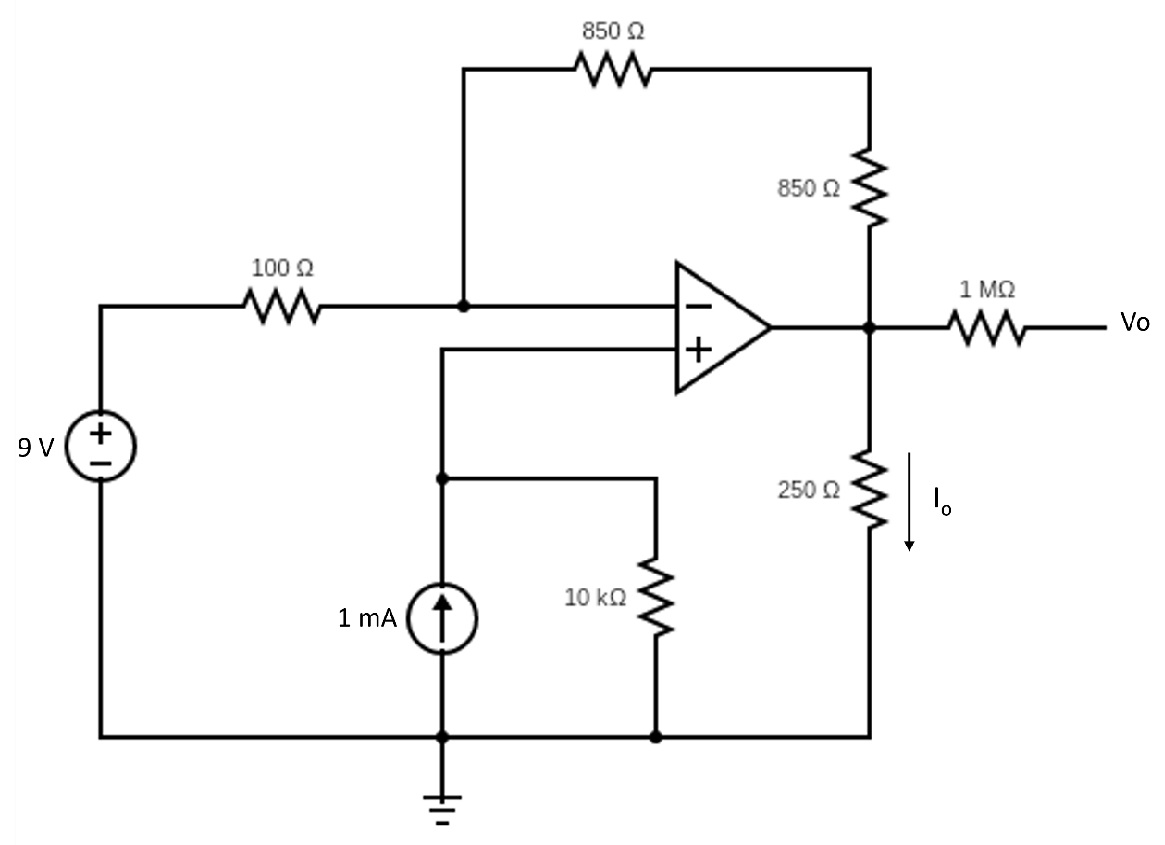
\includegraphics[width=0.7\textwidth]{Fig_OP2.jpg}
		\vspace{-4mm}
		\caption{Circuit for Problem~\ref{pb:op2}.}
		\label{fig:op2}
	\end{figure}
\end{prob}

\noindent\makebox[\linewidth]{\color{rouge_poly}{\rule{\textwidth}{1.3pt}}}

\begin{solprob} \text{}\\
    Let's begin by completing a source transformation to simplify the circuit.
    \[V_\text{1mA} = (1\text{ mA})(10k\Omega) = 10 \text{V}\]
    Let's also combine the two resistors in series.
    \[R_\text{eq1} = 850\Omega + 850 \Omega = 1700 \Omega\]
    Now, again, we know that $V_n=V_p$ and $V_p = 10$ V, so $V_n = 10$ V. Now, lets write a KCL.
    \[\frac{V_x-V_n}{1700} + \frac{9-V_n}{100}=0\]
    \[\frac{V_x-10}{1700} + \frac{9-10}{100}=0\]
    \[V_x-10-17=0\]
    \[V_x=27 \text{ V}\]
    Now, we can solve for $i_o$ using Ohm's law.
    \[i_o = \frac{27}{250}=0.108 \text{ A}\]
\end{solprob}
\vspace{-4mm}
\noindent\makebox[\linewidth]{\color{rouge_poly}{\rule{\textwidth}{1.3pt}}}	

%%%% Final Exam (Neda) - Fall 2023
\begin{prob}\label{pb:op3}\text{}
	Find the output voltage $V_o$ for the circuit shown in Fig.~\ref{fig:op3}.
	
	\begin{figure}[H]
		\centering
		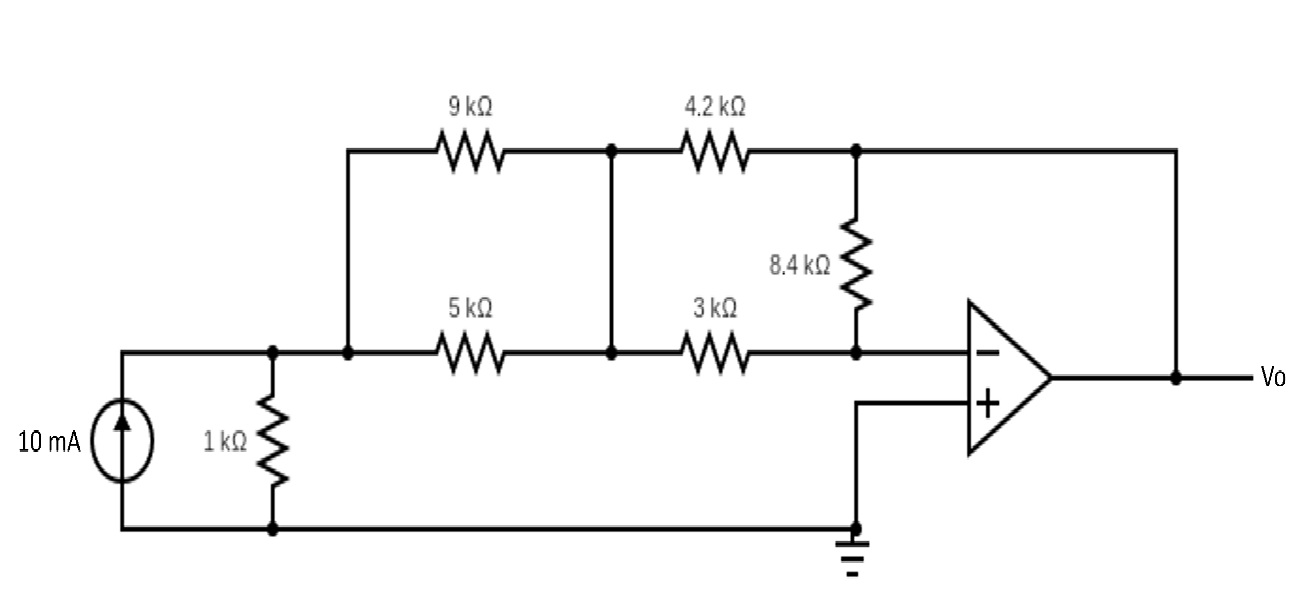
\includegraphics[width=0.7\textwidth]{Fig_OP3.jpg}
		\vspace{-4mm}
		\caption{Circuit for Problem~\ref{pb:op3}.}
		\label{fig:op3}
	\end{figure}
\end{prob}

\noindent\makebox[\linewidth]{\color{rouge_poly}{\rule{\textwidth}{1.3pt}}}

\begin{solprob} \text{}\\
    Let's begin by completing a source transformation and combining the two resistors on the top in parallel and the resulting resistors in series.
    \[V_\text{10mA} = (10\text{ mA})(1\text{ k}\Omega)=10 \text{V}\]
    \[R_\text{eq1}=9k\Omega||5k\Omega=3214 \Omega\]
    \[R_\text{eq2} = 3214 \Omega + 1000\Omega = 4214 \Omega\]
    Now, let's write a KCL.
    \[V_p=V_n = 0\]
    \[\frac{10-V_1}{4214} + \frac{V_o-V_1}{4.2k}=\frac{V_n-V_1}{3k}\]
    \[\frac{10-V_1}{4214}+\frac{V_o-V_1}{4.2k}+\frac{-V_1}{3k}=0\]
    Now, lets write another one.
    \[\frac{V_o-0}{8400}+\frac{V_1-0}{3000}=0\]
    \[V_o+2.8V_1=0\]
    \[V_o=-2.8V_1\]
    Now, lets go back to our first KCL and solve for $V_o$.
    \[\frac{10-V_1}{4214}+\frac{-3.8V_1}{4.2k}-\frac{V_1}{3k}=0\]
    \[10-V_1-1.003(3.8V_1)-1.4046V_1=0\]
    \[-6.216V_1+10=0\]
    \[V_1=1.608 \text{ V}\]
    Now solve for $V_o$ using $V_1$.
    \[V_o=-2.8V_1=-4.50 \text{ V}\]
\end{solprob}
\vspace{-4mm}
\noindent\makebox[\linewidth]{\color{rouge_poly}{\rule{\textwidth}{1.3pt}}}	

%%%% IUT HW6
\begin{prob}\label{pb:op4}\text{}
For the circuit shown in Fig.~\ref{fig:op4}, determine the gain $g=\dfrac{v_o}{v_i}$ in terms of $R_1$, $R_2$, and $R_G$.
	
\vspace{-4mm}
	\begin{figure}[H]
		\centering
		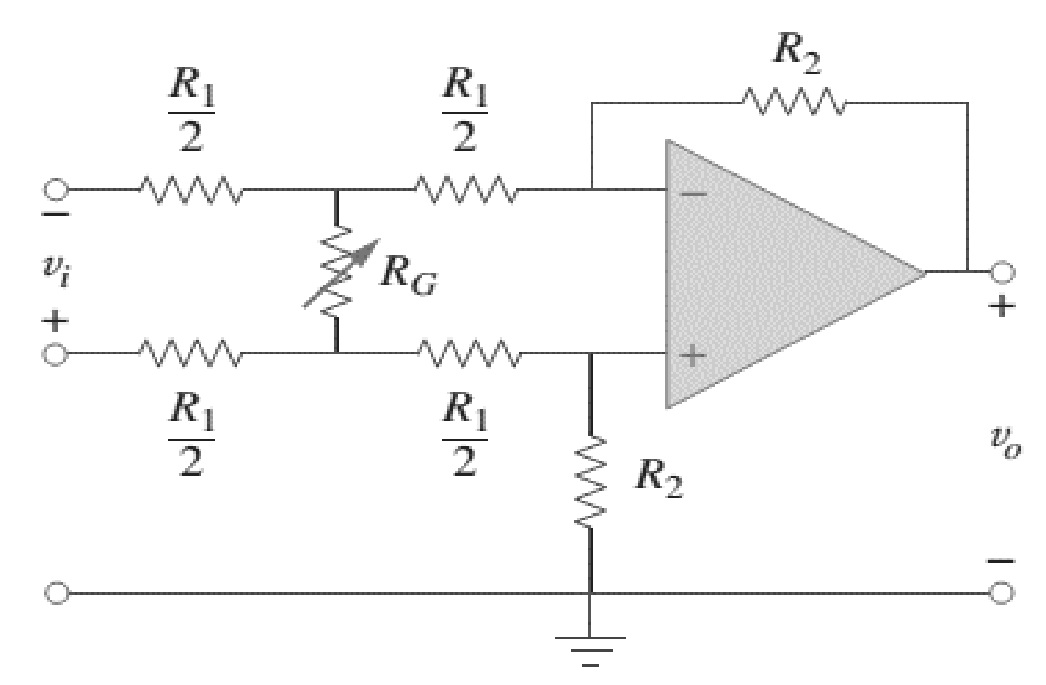
\includegraphics[width=0.6\textwidth]{Fig_OP4.jpg}
		\caption{Adjustable-gain op-amp circuit for Problem~\ref{pb:op4}.}
		\label{fig:op4}
	\end{figure}
\end{prob}

\noindent\makebox[\linewidth]{\color{rouge_poly}{\rule{\textwidth}{1.3pt}}}

\begin{solprob} \text{}\\
    Based on visual analysis, we can determine that this circuit is a non-inverting operational amplifier with an potentiometer connecting each side of the op-amp, creating an adjustable feedback network.  Let's solve for $R_\text{eq}$ when the bottom branch is reduced due to the potentiometer:
    \[R_\text{eq}=\frac{R_GR_1}{2R_G+R_1}\]
    We know that the gain of this ideal op amp circuit is equivalent to:
    \[\frac{v_o}{v_i}=1+\frac{R_f}{R_G}=1+\frac{R_2}{R_\text{eq}}\]
    Therefore, the gain of the circuit is:
    \[\frac{v_o}{v_i}=1+\frac{R_2(2R_G+R_1)}{R_GR_1}\]
\end{solprob}

\noindent\makebox[\linewidth]{\color{rouge_poly}{\rule{\textwidth}{1.3pt}}}	

\begin{prob}\label{pb:op5}\text{}
	Find the input resistance $R_{\text{in}} = \dfrac{V_{\text{in}}}{I_{\text{in}}}$ for the circuit shown in Fig.~\ref{fig:op5}.
	\vspace{-4mm}
	\begin{figure}[H]
		\centering
		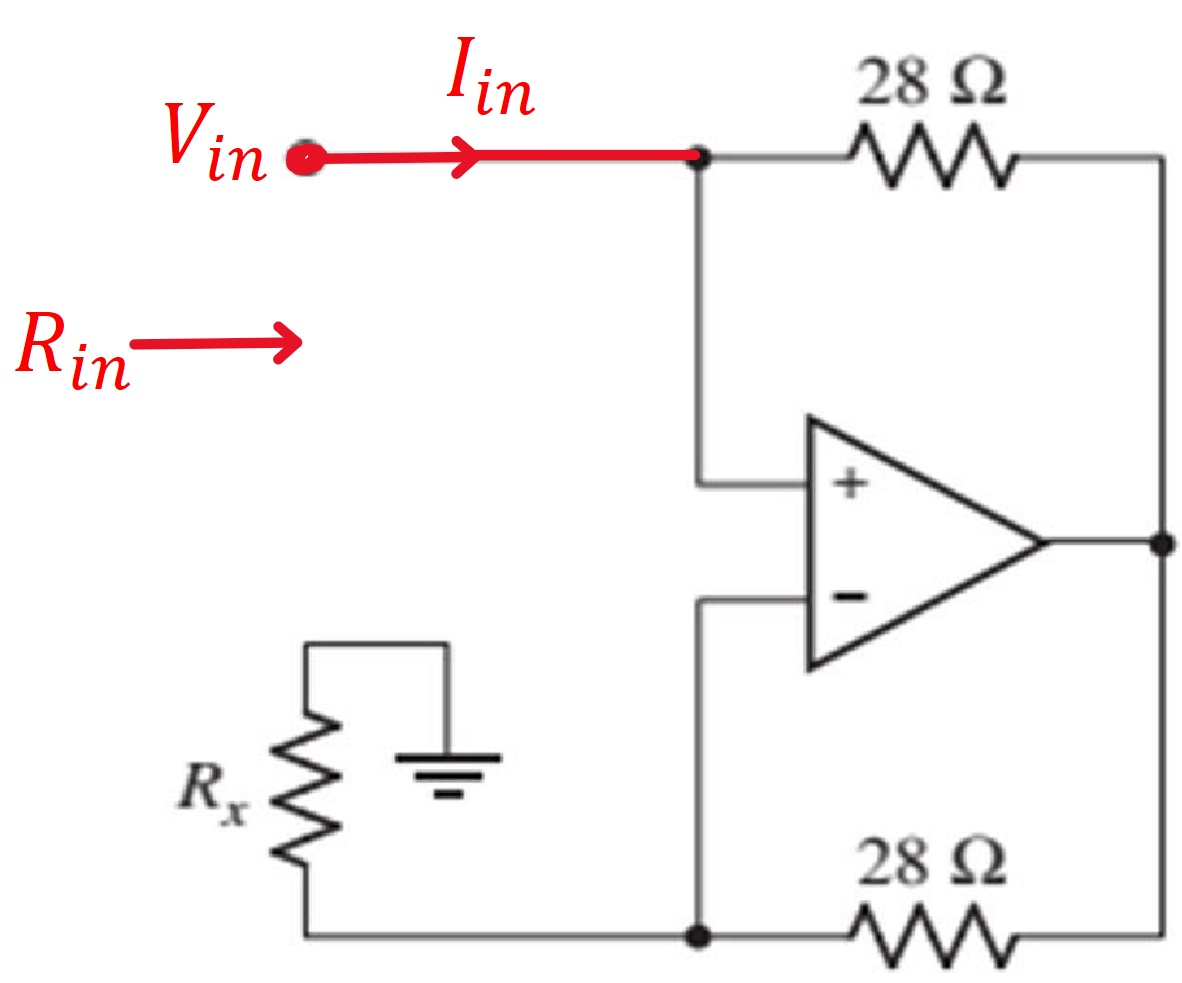
\includegraphics[width=0.4\textwidth]{Fig_OP5.jpg}
		\caption{Circuit for Problem~\ref{pb:op5}.}
		\label{fig:op5}
	\end{figure}
\end{prob}

\noindent\makebox[\linewidth]{\color{rouge_poly}{\rule{\textwidth}{1.3pt}}}

\begin{solprob} \text{}\\
    We begin by noticing that $v_p=v_n$.  We can set $v_p = v_\text{in}$ and therefore, the voltage in the bottom node is equal to $v_\text{in}$. Now, let's take a KCL on the bottom node.
    \[\frac{v_n}{R_x}+\frac{v_n-v_o}{28}=0\]
    \[\frac{v_n}{R_x}=\frac{v_o-v_n}{28}\]
    \[v_o=v_n+\frac{28v_n}{R_x}\]
    \[\therefore v_o = v_\text{in}(1+\frac{28}{R_x})\]
    Since we know that $i_p=i_n=0$, we know that $I_\text{in}$ is equal to the current over the top resistor.
    \[I_\text{in}=\frac{v_p-v_o}{28}=\frac{v_\text{in}-v_\text{in}(1+\frac{28}{R_x})}{28}=-\frac{v_\text{in}}{R_x}\]
    \[\therefore R_\text{in}=-\frac{v_\text{in}}{I_\text{in}}=-R_x\]
    But if we disregard signage:
    \[R_\text{in}=\frac{v_\text{in}}{I_\text{in}}=R_x\]
\end{solprob}

\noindent\makebox[\linewidth]{\color{rouge_poly}{\rule{\textwidth}{1.3pt}}}	
%% Nilsson 12th ed P6.1
\begin{prob}\label{pb:L1}\text{}
	The voltage across a $300~\mu\mathrm{H}$ inductor in Fig.~\ref{fig:L1}(a) is shown in Fig.~\ref{fig:L1}(b). The inductor current $i$ is known to be zero for $t \le 0$.
	
	\begin{enumerate}[label=(\alph*)]
		\item Derive the expression for $i$ for $t \ge 0$.
		\item Sketch $i$ versus $t$ for $0 \le t \le \infty$.
	\end{enumerate}
	
	\vspace{-3mm}
	\begin{figure}[H]
		\centering
		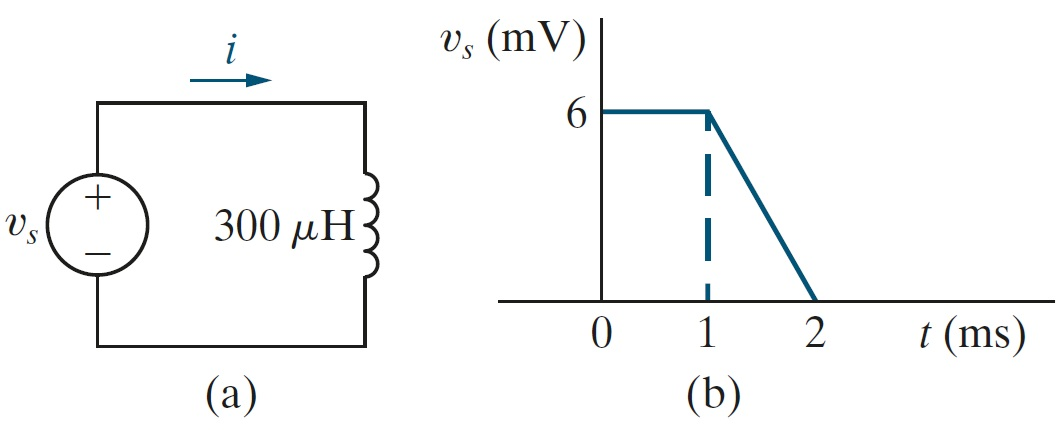
\includegraphics[width=0.55\textwidth]{Fig_L1.jpg}
		\caption{Inductor voltage for Problem~\ref{pb:L1}.}
		\label{fig:L1}
	\end{figure}
\end{prob}

\noindent\makebox[\linewidth]{\color{rouge_poly}{\rule{\textwidth}{1.3pt}}}

\begin{solprob} \text{}\\
    (a)Let's begin by writing a KVL:
    \[\text{KVL: }-V_s+V_L=0\]
    \[V_s=L\frac{di}{dt}\]
    \[\frac{di}{dt}=\frac{V_s}{L}\]
    \[\int{}{}di=\int{}{}\frac{V_s}{L}dt=\frac{V_s}{L}t+I(t_0)\]
    \[\therefore I(t)=\frac{V_s}{L}t+I(t_0)\]
    (b)\begin{figure}[H]
    		\centering
    		\includegraphics[width=0.70\textwidth]{IMG_0304.png}
    		\caption{i vs. t graph for Part (b).}
    		\label{fig:L1}
    	\end{figure}
\end{solprob}

\noindent\makebox[\linewidth]{\color{rouge_poly}{\rule{\textwidth}{1.3pt}}}	

%% Nilsson 12th ed P6.7
\begin{prob}\label{pb:Triangle}\text{}
	The triangular current pulse shown in Fig.~\ref{fig:Triangle} is applied to a $375~\mathrm{mH}$ inductor.
	
	\begin{enumerate}[label=(\alph*)]
		\item Write the expressions that describe $i(t)$ in the four intervals:
		$t < 0$, $0 \le t \le 25~\mathrm{ms}$, $25~\mathrm{ms} \le t \le 50~\mathrm{ms}$, and $t > 50~\mathrm{ms}$.
		\item Derive the expressions for the inductor voltage, power, and energy using the passive sign convention.
	\end{enumerate}
	
	\vspace{-3mm}
	\begin{figure}[H]
		\centering
		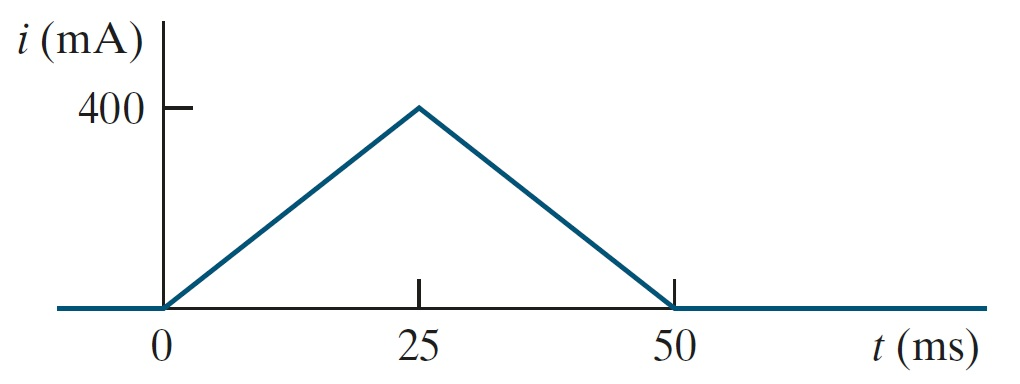
\includegraphics[width=0.55\textwidth]{Fig_Triangle.jpg}
		\caption{Triangular current pulse for Problem~\ref{pb:Triangle}.}
		\label{fig:Triangle}
	\end{figure}
\end{prob}

\noindent\makebox[\linewidth]{\color{rouge_poly}{\rule{\textwidth}{1.3pt}}}

\begin{solprob} \text{}\\
    (a)
    \begin{equation}
    i(t)=\begin{cases}
    0 & \text{if } t<0\\
    16t & \text{if } 0\leq t\leq 0.025\\
    0.8-16t & \text{if } 0.025\leq t \leq 0.050\\
    0 & \text{if } t>0.050
    \end{cases}
    \end{equation}
    (b)
    \begin{equation}
    V_L(t)=\begin{cases}
    0 & \text{if } t<0\\
    L\frac{di}{dt}=0.375(16)=6\text{ V} & \text{if } 0\leq t \leq0.025\\
    L\frac{di}{dt}=0.375(-16)=-6 \text{ V} & \text{if } 0.025\leq t \leq 0.050\\
    0 & \text{if } t>0.050
    \end{cases}
    \end{equation}
    \begin{equation}
    p(t)=\begin{cases}
    0 & \text{if } t<0\\
    6(16t)=96t & \text{if } 0\leq t\leq 0.025\\
    (-6)(0.8-16t)=-4.8+96t & \text{if } 0.025\leq t\leq 0.050\\
    0 & \text{if } t>0.050
    \end{cases}
    \end{equation}
    \begin{equation}
    W_L(t)=\begin{cases}
    0 & \text{if } t<0\\
    \frac{1}{2}(0.375)(16t)^2=48t^2 & \text{if } 0\leq t\leq 0.025\\
    \frac{1}{2}(0.375)(0.8-16t)^2 & \text{if } 0.025\leq t\leq 0.050\\
    0 & \text{if } t>0.050
    \end{cases}
    \end{equation}
\end{solprob} 

\noindent\makebox[\linewidth]{\color{rouge_poly}{\rule{\textwidth}{1.3pt}}}	

\vspace{-5mm}

%% Alex 7th ed P6.77
\begin{prob}\label{pb:OPRC}\text{}
	The output voltage $v_o$ of the op-amp circuit in Fig.~\ref{fig:OPRC}(a) is shown in Fig.~\ref{fig:OPRC}(b). Let $R_i = R_f = 1~\text{M}\Omega$ and $C = 1~\mu\text{F}$. Determine the input voltage waveform and sketch it.
	
	\vspace{-3mm}
	\begin{figure}[H]
		\centering
		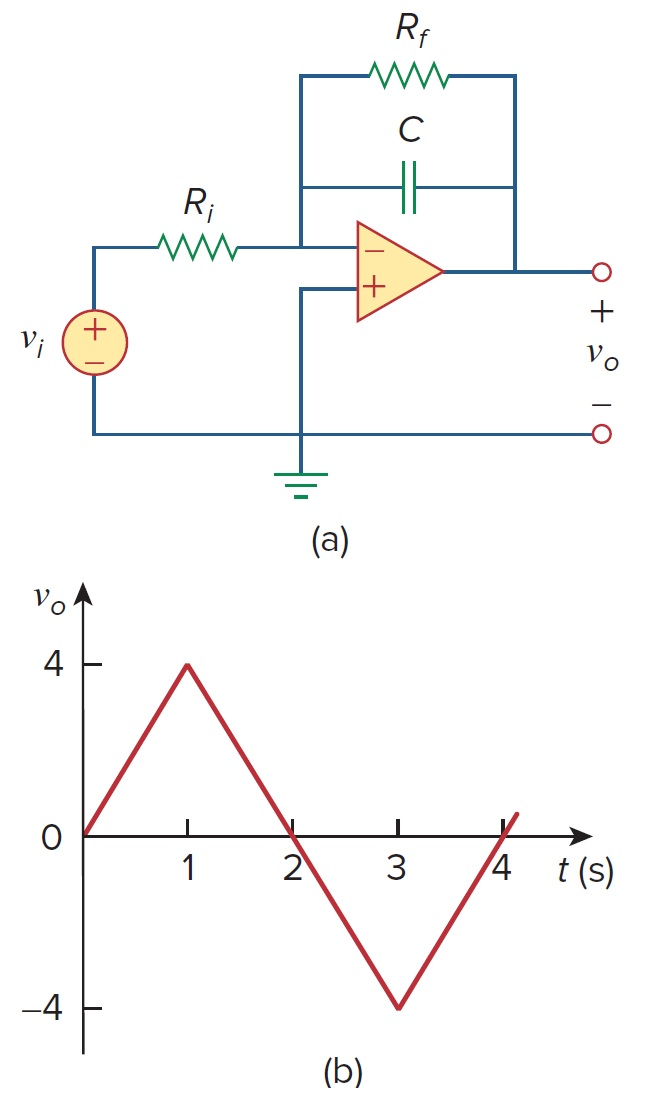
\includegraphics[width=0.4\textwidth]{Fig_OP_RC.jpg}
		\caption{Op-amp circuit and output waveform for Problem~\ref{pb:OPRC}.}
		\label{fig:OPRC}
	\end{figure}
\end{prob}

\noindent\makebox[\linewidth]{\color{rouge_poly}{\rule{\textwidth}{1.3pt}}}

\begin{solprob} \text{}\\
    Let's begin with a KCL:
    \[\text{KCL: } i_i=i_f+i_c\]
    \[\frac{V_1-0}{R_i}=\frac{0-V_o}{R_f}+C\frac{dV_o}{dt}\]
    \[RC = 1*10^6(1*10^\text{-6})=1\]
    \[v_=-R_i(\frac{V_o}{R_f}+C\frac{dV_o}{dt} = -(V_o + \frac{dV_o}{dt})\]
    
    \begin{figure}[H]
        \centering
        \includegraphics[width=0.30\textwidth]{IMG_0305.png}
        \caption{i vs. t graph for Part (b).}
        \label{fig:L1}
    \end{figure}
\end{solprob}

\noindent\makebox[\linewidth]{\color{rouge_poly}{\rule{\textwidth}{1.3pt}}}	
%% Alex 7th ed P6.57
\begin{prob}\label{pb:Leq}\text{}
	Determine the equivalent inductance $L_{\mathrm{eq}}$ that can represent the inductive network of Fig.~\ref{fig:Leq} at the given terminals.
	
	\vspace{-3mm}
	\begin{figure}[H]
		\centering
		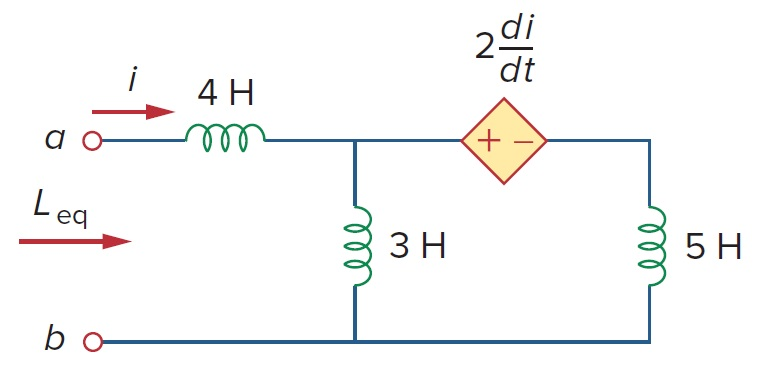
\includegraphics[width=0.5\textwidth]{Fig_Leq.jpg}
		\caption{Inductive network for Problem~\ref{pb:Leq}.}
		\label{fig:Leq}
	\end{figure}
\end{prob}

\noindent\makebox[\linewidth]{\color{rouge_poly}{\rule{\textwidth}{1.3pt}}}

\begin{solprob} \text{}\\
    Let's begin with a KCL.
    \[\text{KCL: } i=i_1+i_2\]
    Also, we should define the two equations for the voltage in parallel.
    \[V_2=\frac{3di}{dt}\implies\frac{di_1}{dt} =\frac{V_2}{3}\]
    \[V_2=\frac{2di}{dt}+\frac{5di_2}{dt}\]
    Now, back to the KCL:
    \[V_2=2\frac{di}{dt}+5\frac{di}{dt}-5\frac{di}{dt}=7\frac{di}{dt}-5\frac{di_1}{dt}=7\frac{di}{dt}+5\frac{V_2}{3}\]
    \[V_2+5\frac{V_2}{3}=7\frac{di}{dt}\]
    \[\frac{8}{3}V_2=7\frac{di}{dt}\]
    \[V_2=\frac{21}{8}\frac{di}{dt}\]
    \[V=4\frac{di}{dt}+\frac{21}{8}\frac{di}{dt}=frac{32}{8}\frac{di}{dt}+\frac{21}{8}\frac{di}{dt}=\frac{53}{8}\frac{di}{dt}=6.675\frac{di}{dt}\]
    \[L_\text{eq}=6.625 \text{ H}\]
\end{solprob}

\noindent\makebox[\linewidth]{\color{rouge_poly}{\rule{\textwidth}{1.3pt}}}	

%% Nilsson 12th ed P6.17
\begin{prob}\label{pb:CapPiecewise}\text{}
	The voltage across a $400~\text{nF}$ capacitor is
	\[
	v(t)=
	\begin{cases}
		25~\text{V}, & t\le 0,\\[2mm]
		A_1 t\,e^{-1500t}+A_2 e^{-1500t}\ \text{V}, & t\ge 0.
	\end{cases}
	\]
	The initial capacitor current is $90~\text{mA}$ (passive sign convention).
	
	\begin{enumerate}[label=(\alph*)]
		\item Find the initial energy stored in the capacitor.
		\item Determine the coefficients $A_1$ and $A_2$.
		\item Write the expression for the capacitor current $i(t)$.
	\end{enumerate}
\end{prob}

\noindent\makebox[\linewidth]{\color{rouge_poly}{\rule{\textwidth}{1.3pt}}}

\begin{solprob} \text{}\\
    (a) \[W_c(0)=\frac{1}{2}CV(0) = \frac{1}{2}(4*10^\text{-7})(25)^2=1.25*10^\text{-4} J\]
    (b)
    \[V(t)=A_1te^\text{-1500t}+A_2e^\text{-1500t}=e^\text{-1500t}(A_1t+A_2)\]
    \[V(0)=A_2=25\text{ V}\]
    \[\frac{dv}{dt}=-1500e^\text{-1500t}(A_1t+A_2) + e^\text{-1500t}A_1=(-1500A_1t-1500A_2+A_1)e^\text{-1500t}\]
    \[\frac{dv(0)}{dt} = A_1-1500A_2\]
    \[i=C\frac{dv}{dt} \,\,\,\,\,\,\,\,\,\,\,\,\,\,\,\,\,\,\,\,\,\,\,i(0)=C\frac{dv(0)}{dt}\]
    \[\frac{dv(0)}{dt}=\frac{i(0)}{C}=\frac{90*10^\text{-3}}{4*10^\text{-7}}=225000\]
    \[225000 = A_1-1500(25) \implies A_1 = 187500\]

    (c)\[V=(187500t+25)e^\text{-1500(25)}\]
    \[i=C\frac{dv}{dt}=4*10^\text{-7}\frac{d}{dt}(187500t+25)e^\text{-1500t}\]
    \[i=4*10^\text{-7}(187500e^\text{-1500t}-1500(187500t+25)e^\text{-1500t})=(0..09-157.5t)e^\text{-1500t})\]
    
\end{solprob}

\noindent\makebox[\linewidth]{\color{rouge_poly}{\rule{\textwidth}{1.3pt}}}	

%% Nilsson 12th ed P6.26
\begin{prob}\label{pb:ThreeL}\text{}
	The three inductors in Fig.~\ref{fig:ThreeL} are connected across the terminals of a black box at $t=0$. The resulting voltage for $t>0$ is
	\[
	v_o(t)=1250\,e^{-25t}\ \text{V}.
	\]
	Given $i_1(0)=10~\text{A}$ and $i_2(0)=-5~\text{A}$, find:
	\begin{enumerate}[label=(\alph*)]
		\item $i_o(0)$;
		\item $i_o(t)$, $t\ge 0$;
		\item $i_1(t)$, $t\ge 0$;
		\item $i_2(t)$, $t\ge 0$;
		\item the initial energy stored in the three inductors;
		\item the total energy delivered to the black box; and
		\item the energy trapped in the ideal inductors.
	\end{enumerate}
	
	\vspace{-3mm}
	\begin{figure}[H]
		\centering
		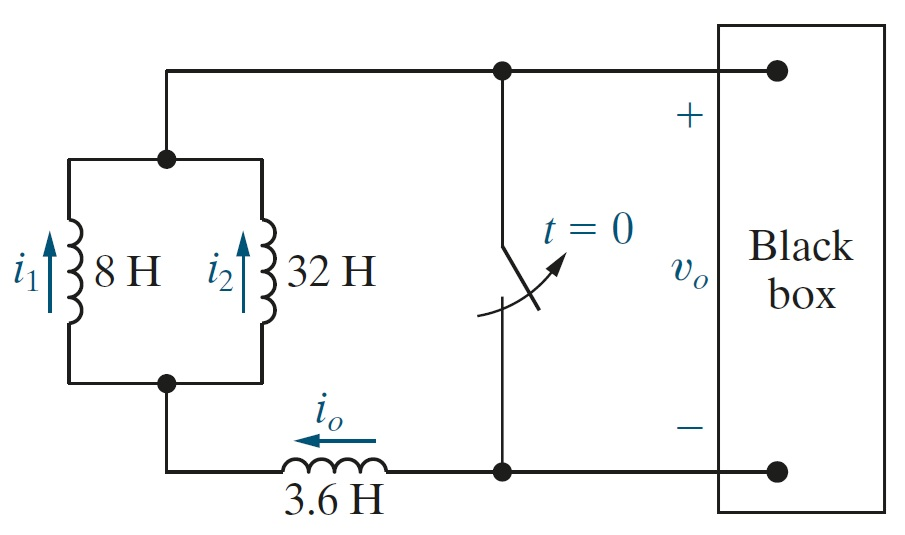
\includegraphics[width=0.58\textwidth]{Fig_3L.jpg}
		\caption{Inductor network for Problem~\ref{pb:ThreeL}.}
		\label{fig:ThreeL}
	\end{figure}
\end{prob}

\noindent\makebox[\linewidth]{\color{rouge_poly}{\rule{\textwidth}{1.3pt}}}	

\begin{solprob} \text{}\\
    \[V_o=V_1+V_2\,\,\,\,\,\,\,\,\,\,\,\,\,\,\,\,\,\,\, V_1=L\frac{di_o}{dt}\]
    (a) \[i_o=i_1+i_2\,\,\,\,\,\,\,\,\,\,\,\,\,\,\,\,\,\,\,i_o(0)=i_1(0)+i_2(0)=10-5=5\text{ A}\]
    (b)\[L_\text{eq1}=8H||32H=\frac{8(32)}{8+32}=6.4 \text{ H}\]
    \[L_\text{eq}=3.6+6.4 = 10\text{ H}\]
    \[V_o(t)=L_\text{eq}\frac{di_o}{dt} \implies \frac{di_o}{dt}=\frac{1250}{10}e^\text{-25t}=125e^\text{-25t}\]
    \[i_o(t)=i_o(0)+[\frac{-125}{25}e^\text{-25$\tau$}]^t_0=5t(-5e^\text{25t}+5=10-5e^\text{-25t}\]
    (c)\[i_1(t)=i_1(0)+\frac{1}{8}\int^t_0v_p(\tau)d\tau\]
    \[i_2=i_2(0)+\frac{1}{32}\int^t_0v_p(\tau)d\tau\]
    \[i_1(t)-i_2(t)=i_1(0)-4i_2(0) = 10-4(-5)=30\]
    \[i_1=i_o-i_2 \implies i_2=i_o-i_1\]
    \[i_o-5i_2=30\implies i_2=0.2i_o-6=2-6-e^\text{-25t}=-4-e^\text{-25t}\]
    (d)\[i_1-4(i_o-i_1)=30\implies i_1+4i_1-4i_o=30\implies i_1=0.8i_o+6=8+6+4e\text{-25t}=14+4e^\text{-25t}\]
    (e) \[W_L(0)=\frac{1}{2}(8)(10)^2+\frac{1}{2}(32)(-5)^2+\frac{1}{2}(3.6)(5)^2=400+400+45=845\text{ J}\]
    (f)\[i_o(\infty)=10\text{ A}, i_1(\infty)=14\text{ A}, i_2(\infty)=-4\text{ A}\]
    \[W(\infty)=\frac{1}{2}(3.6)(10)^2+\frac{1}{2}(8)(14)^2+\frac{1}{2}(32)(-4)^2=784+256+180=1220 \text{ J}\]
    \[\Delta W=W(\infty)-W(0)=1220-845=+375\text{ J}\]
    Energy delivered to the black box would be -$\Delta W = -375$ J
    \\\,\\(g) Energy trapped would be the energy remaining in the circuit as $t\rightarrow0$, so that means $V\rightarrow0$, $\therefore W(\infty) = 1220 \text{ J}$
\end{solprob}

\noindent\makebox[\linewidth]{\color{rouge_poly}{\rule{\textwidth}{1.3pt}}}

%% Dorf 9th ed P 7.8-11
\begin{prob}\label{pb:RLCss}\text{}
	The circuit in Fig.~\ref{fig:RLCss} has reached steady state before the switch opens at $t=0$. Determine $i_L(t)$, $v_C(t)$, and $v_R(t)$ immediately before the switch opens, and find $v_R(t)$ immediately after the switch opens.
	
	\vspace{-3mm}
	\begin{figure}[H]
		\centering
		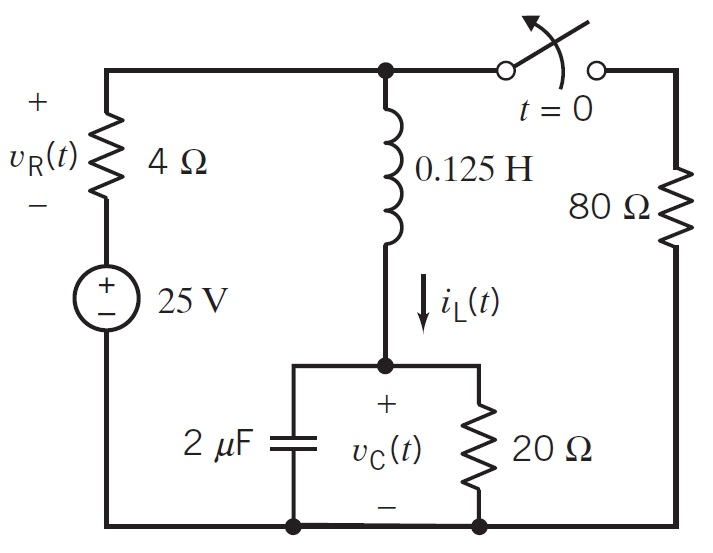
\includegraphics[width=0.5\textwidth]{Fig_RLC_ss.jpg}
		\caption{Circuit for Problem~\ref{pb:RLCss}.}
		\label{fig:RLCss}
	\end{figure}
\end{prob}

\vspace{-5mm}

\noindent\makebox[\linewidth]{\color{rouge_poly}{\rule{\textwidth}{1.3pt}}}	

\begin{solprob} \text{}\\
    In steady state, inductor is short circuit and capacitor is open circuit.
    \[\therefore R_\text{eq1}=80||20=16\Omega\]
    \[R_\text{eq}= 4 + 16 = 20 \Omega\]
    \[I=\frac{25 \text{ V}}{20 \Omega}=1.25 \text{ A}\]
    \[v_c(0)=16(1.25 \text{ A})=20 \text{ A}\]
    \[i_\text{20}=\frac{80}{100}I = 1.25(0.8)=1\text{ A}=i_c(0^-)\]
    \[i_\text{80}=\frac{20}{100}I=0.25\text{ A}\]
    \[v_R=-IR=-(1.25)(4)=-5V\]
    After the switch opens, $I_c$ and $v_C$ cannot change instantaneously, so they are still the same as before right after the switch closes.
    \[v_R(0^+)=\frac{-25+v_\text{top}}{4}+I_L(0^+)=0\]
    \[v_\text{top}=25-4(1\text{ A})=0 \implies v_\text{top}=21 \text{ V}\]
    \[\therefore v_R=21-25=-4\text{ V}\]
\end{solprob}

\noindent\makebox[\linewidth]{\color{rouge_poly}{\rule{\textwidth}{1.3pt}}}

%% Dorf 9th ed P 7.5-20
\begin{prob}\label{pb:L}\text{}
	Consider the inductor in Fig.~\ref{fig:L}. The current and voltage are
	\[
	i(t)=
	\begin{cases}
		5t-4.6, & 0\le t\le 0.2,\\[2mm]
		at+b, & 0.2\le t\le 0.5,\\[2mm]
		c, & t\ge 0.5,
	\end{cases}
	\qquad
	v(t)=
	\begin{cases}
		12.5, & 0<t<0.2,\\[2mm]
		25, & 0.2<t<0.5,\\[2mm]
		0, & t>0.5,
	\end{cases}
	\]
	where $a$, $b$, and $c$ are real constants. The current is given
	in amps, the voltage in volts, and the time in seconds. Determine $L$, $a$, $b$, and $c$.
	
	\vspace{-3mm}
	\begin{figure}[H]
		\centering
		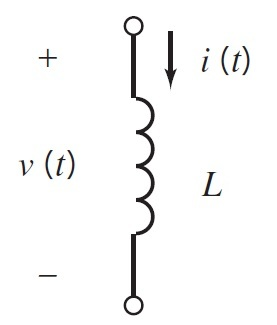
\includegraphics[width=0.2\textwidth]{Fig_L.jpg}
		\caption{Inductor for Problem~\ref{pb:L}.}
		\label{fig:L}
	\end{figure}
\end{prob}

\noindent\makebox[\linewidth]{\color{rouge_poly}{\rule{\textwidth}{1.3pt}}}

\begin{solprob} \text{}\\
    \[V=L\frac{di}{dt}\implies 12.5=L(5)\implies L=\frac{12.5}{5}=2.5\]
    \[25=2.5a \implies a=10\]
    \[5t-4.6=at+b,t=0.2 \implies1-4.6=10(0.2)+b\implies-3.6-2=b\implies b=-5.6\]
    \[c=10(0.5)-5.6=5-5.6=-0.6 \text{ A}\]
\end{solprob}

\vspace{-5mm}

\noindent\makebox[\linewidth]{\color{rouge_poly}{\rule{\textwidth}{1.3pt}}}	

%% Nilsson 12th ed P6.39
\begin{prob}\label{pb:LM}\text{}
	Two magnetically coupled coils are connected in parallel between terminals $a$ and $b$ as in Fig.~\ref{fig:LM}.  
	
	\begin{enumerate}[label=(\alph*)]
		\item Show that the pair can be replaced by a single inductor of inductance
		\[
		L_{ab}=\frac{L_1L_2-M^2}{L_1+L_2-2M}.
		\]
		
		\item If the magnetic polarity of coil 2 is reversed (i.e., the dot on coil 2 is moved to the opposite terminal), show that
		\[
		L_{ab}=\frac{L_1L_2-M^2}{L_1+L_2+2M}.
		\]
	\end{enumerate}
	
	\vspace{-3mm}
	\begin{figure}[H]
		\centering
		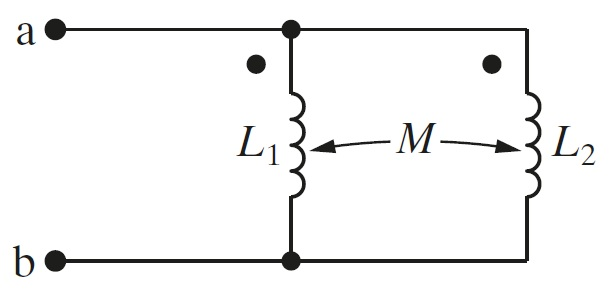
\includegraphics[width=0.45\textwidth]{Fig_LM.jpg}
		\caption{Parallel-coupled inductors for Problem~\ref{pb:LM}.}
		\label{fig:LM}
	\end{figure}
\end{prob}

\noindent\makebox[\linewidth]{\color{rouge_poly}{\rule{\textwidth}{1.3pt}}}	

\begin{solprob} \text{}\\
     (a) Let's begin with the mesh-current method, defining the left mesh as mesh 1 and right mesh as mesh 2.
     \[\text{Mesh 1: } v_\text{ab}=L_1\frac{d(i_1-i_2)}{dt}+M\frac{di_2}{dt}\]
     \[\text{Mesh 2: } L_1\frac{d(i_2-i_1)}{dt}-M\frac{di_2}{dt}+L_2\frac{di_2}{dt}-M\frac{d(i_2-i_1}{dt}=0\]
     Let's focus on the second equation.
     \[L_1(\frac{di_2}{dt}-\frac{di_1}{dt})-M\frac{di_2}{dt}+L_2\frac{di_2}{dt}-M(\frac{di_2}{dt}-\frac{di_2}{dt})=0\]
     \[\frac{di_2}{dt}(L_1+L_2-2M)+\frac{di_1}{dt}(M-L_1)=0\]
     \[\frac{di_2}{dt}=\frac{di_1}{dt}(\frac{L_1-M}{L_1+L_2+2M})\]
     We have simplified this mesh enough, so now lets go back to the first equation.
     \[v_\text{ab}=L_1\frac{di_1}{dt}+\frac{di_2}{dt}(M-L_1)\]
     \[v_\text{ab}=L_1\frac{di_1}{dt}+\frac{di_1}{dt}(\frac{L_1-M(M-L_1)}{L_1+L_2-2M})\]
     \[v_\text{ab}=\frac{di_1}{dt}(L_1+\frac{L_1M-L_1\,^2-M^2+L_1M}{L_1+L_2-2M})\]
     \[v_\text{ab}=\frac{di_1}{dt}(\frac{L_1(L_1+L_2-2M)+2L_1M-L_1\,^2-M^2}{L_1+L_2-2M})\]
     \[v_\text{ab}=\frac{di_1}{dt}(\frac{L_1\,^2+L_1L_2-2L_1M+2L_1M-L_1\,^2-M^2}{L_1+L_2-2M})\]
     \[v_\text{ab}=\frac{di_1}{dt}(\frac{L_1L_2-M^2}{L_1+L_2-2M})\]
     \[\therefore L_\text{ab}=\frac{L_1L_2-M^2}{L_1+L_2-2M}\]
     (b) Let's begin with the same method again.
     \[\text{Mesh 1: } v_\text{ab}=L_1\frac{d(i_1-i_2)}{dt}-M\frac{di_2}{dt}\]
     \[\text{Mesh 2: } L_1\frac{d(i_2-i_1)}{dt}+M\frac{di_2}{dt}+L_2\frac{di_2}{dt}+M\frac{d(i_2-i_1)}{dt}=0\]
     Let's again work equation 2:
     \[\frac{di_2}{dt}(L_1+M+L_2+M)+\frac{di_1}{dt}(-M-L_1)\]
     \[\frac{di_2}{dt}=\frac{di_1}{dt}(\frac{M+L_1}{L_1+L_2+2M})\]
     Now, lets substitute this back into equation 1.
     \[v_\text{ab}=L_1\frac{di_1}{dt}+\frac{di_2}{dt}(-M-L_1)\]
     \[v_\text{ab}=L_1\frac{di_1}{dt}+\frac{-(-M-L_1)^2}{L_1+L_2+2M}\frac{di_1}{dt}\]
     \[v_\text{ab}=\frac{di_1}{dt}(L_1-\frac{M^2+2L_1M+L_1\,^2}{L_1+L_2+2M})\]
     \[v_\text{ab}=\frac{di_1}{dt}(\frac{L_1\,^2+L_1L_2+2L_1M-(M^2+2L_1M+L_1\,^2)}{L_1+L_2+2M})\]
     \[v_\text{ab}=(\frac{L_1L_2-M^2}{L_1+L_2+2M})\frac{di_1}{dt}\]
     \[\therefore L_\text{ab}=\frac{L_1L_2-M^2}{L_1+L_2+2M}\]
\end{solprob}

\noindent\makebox[\linewidth]{\color{rouge_poly}{\rule{\textwidth}{1.3pt}}}	

%% Dorf 9th ed P 7.8-1
\begin{prob}\label{pb:RLC1}\text{}
	The switch in Fig.~\ref{fig:RLC1} has been open for a long time before closing at $t=0$.
	Let $v_c(0^+)$ and $i_L(0^+)$ denote the capacitor voltage and inductor current immediately after the switch closes, and let $v_c(\infty)$ and $i_L(\infty)$ denote their values after the switch has been closed for a long time.
	
	\begin{enumerate}[label=(\alph*)]
		\item Find $v_c(0^+)$ and $i_L(0^+)$.
		\item Find $v_c(\infty)$ and $i_L(\infty)$.
	\end{enumerate}
	
	\vspace{-3mm}
	\begin{figure}[H]
		\centering
		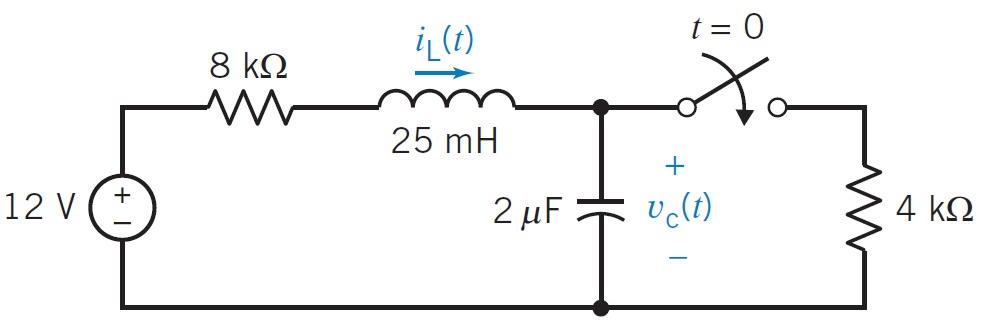
\includegraphics[width=0.65\textwidth]{Fig_RLC1.jpg}
		\caption{Circuit for Problem~\ref{pb:RLC1}.}
		\label{fig:RLC1}
	\end{figure}
\end{prob}

\noindent\makebox[\linewidth]{\color{rouge_poly}{\rule{\textwidth}{1.3pt}}}

\begin{solprob} \text{}\\
    (a) Since the circuit is in steady state, you can open circuit the capacitor and short circuit the inductor. $\therefore$ just after the switch closes, the voltage is the same everywhere in the circuit and the current remains 0, so
    \[v_c(0^+) = 12 \text{ V} \,\,\,\,\,\,\,\, i_L(0^+) = 0 \text{ A}\]
    (b) To solve for $i_L(\infty)$, we need Ohm's law.
    \[i_L(\infty)=\frac{12}{8\text{k} + 4\text{k}}=1\text{ mA}\]
    To solve for $v_c(\infty)$, we use Ohm's law again.
    \[v_c(\infty) = i_L(\infty)(4\text{k}) = 4 \text{ V}\]
\end{solprob}

\noindent\makebox[\linewidth]{\color{rouge_poly}{\rule{\textwidth}{1.3pt}}}	

%% Nilsson 12th ed P6.36
\begin{prob}\label{pb:LC}\text{}
	At $t=0$, a series-connected capacitor and inductor are placed across the terminals of a black box, as shown in Fig.~\ref{fig:LC}.  
	For $t \ge 0$, it is known that
	\[
	i_o = -e^{-80t}\sin(60t)\ \text{A}.
	\]
	If $v_C(0) = -300~\text{V}$, find $v_o$ for $t \ge 0$.
	
	\vspace{-3mm}
	\begin{figure}[H]
		\centering
		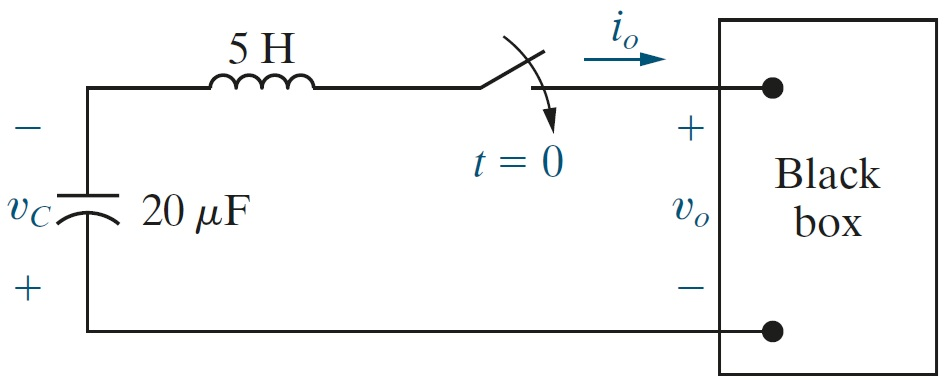
\includegraphics[width=0.55\textwidth]{Fig_LC.jpg}
		\caption{Series $LC$ circuit for Problem~\ref{pb:LC}.}
		\label{fig:LC}
	\end{figure}
\end{prob}


\noindent\makebox[\linewidth]{\color{rouge_poly}{\rule{\textwidth}{1.3pt}}}

\begin{solprob} \text{}\\
    Let's begin by solving for $V_C$.
    \[v_C=\frac{1}{20*10^\text{-6}}\int^t_0-e^\text{-80$\tau$}\sin(60\tau)d\tau+i_o(0)\]
    \[v_C=5e^\text{-80t}[80\sin60t+60\cos60t]-600\]
    \[v_C=400e^\text{-80t}\sin60t+300e^\text{-80t}\cos60t-600\]
    Now, let's find $v_L$.
    \[v_L=L\frac{di_o}{dt}=5\frac{di_o}{dt}\]
    Substitute in the derivative from the given $i_o$.
    \[v_L=5(80e^\text{-80t}\sin60t-60e^\text{-80t}\cos60t)\]
    \[v_L=400e^\text{-80t}\sin60r-300e^\text{-80t}\cos60t\]
    Now, let's solve for $v_o$ using KVL:
    \[v_o=-v_C-v_L\]
    \[v_o=-400e^\text{-80t}\sin60t-300e^\text{-80t}\cos60t+600-400e^\text{-80t}\sin60t+300e^\text{-80t}\cos60t\]
    \[v_o=600-800e^\text{-80t}\cos60t\]
    
\end{solprob}

\end{document}
